\documentclass{article}
\usepackage{graphicx}
\usepackage{geometry}
\usepackage{hyperref}
\usepackage{booktabs}
\usepackage{subcaption}

\geometry{
    a4paper,
    margin=0.8in
}

\hypersetup{
    colorlinks=true,
    linkcolor=blue,
    filecolor=magenta,      
    urlcolor=cyan,
}

\title{Multi-Seed Byzantine Robustness:\\CNN vs. SNN under Extreme Heterogeneity ($\gamma = 0$)}
\author{ByzFL SNN Benchmark}
\date{\today}

\begin{document}

\maketitle

\section{Introduction}
This document presents a statistical robustness evaluation comparing Convolutional Neural Networks (CNNs) and Spiking Neural Networks (SNNs) on the MNIST dataset. The experiments were executed over 5 independent training seeds (seeds 42 to 46) under extreme data heterogeneity ($\gamma = 0.0$ for Non-IID distribution) with $N=16$ honest clients. 

The benchmark compares two architectures:
\begin{enumerate}
    \item \textbf{CNN}: A standard feedforward CNN (\texttt{convnet\_cnn})
    \item \textbf{SNN}: A Spiking CNN (\texttt{convnet\_snn}) with constant rate coding ($T=25$ time steps, threshold $= 1.0$, $\beta=0.95$).
\end{enumerate}

Both architectures are evaluated against the Optimal A Little Is Enough (ALIE) and Optimal Inner Product Manipulation (IPM) attacks across varying numbers of Byzantine workers $f \in \{2, 4, 6, 8\}$, using two state-of-the-art aggregation protocols: Centered Clipping and Geometric Median (pre-aggregated with NNM and ARC).

\newpage

\section{Heatmap Grids of Mean Accuracy}
This section illustrates the aggregated final accuracy heatmaps for CNN and SNN under both attack models. The heatmaps are saved in the directory \texttt{extra\_seeds\_plots/}.

\begin{figure}[htbp]
    \centering
    \begin{subfigure}[b]{0.85\textwidth}
        \centering
        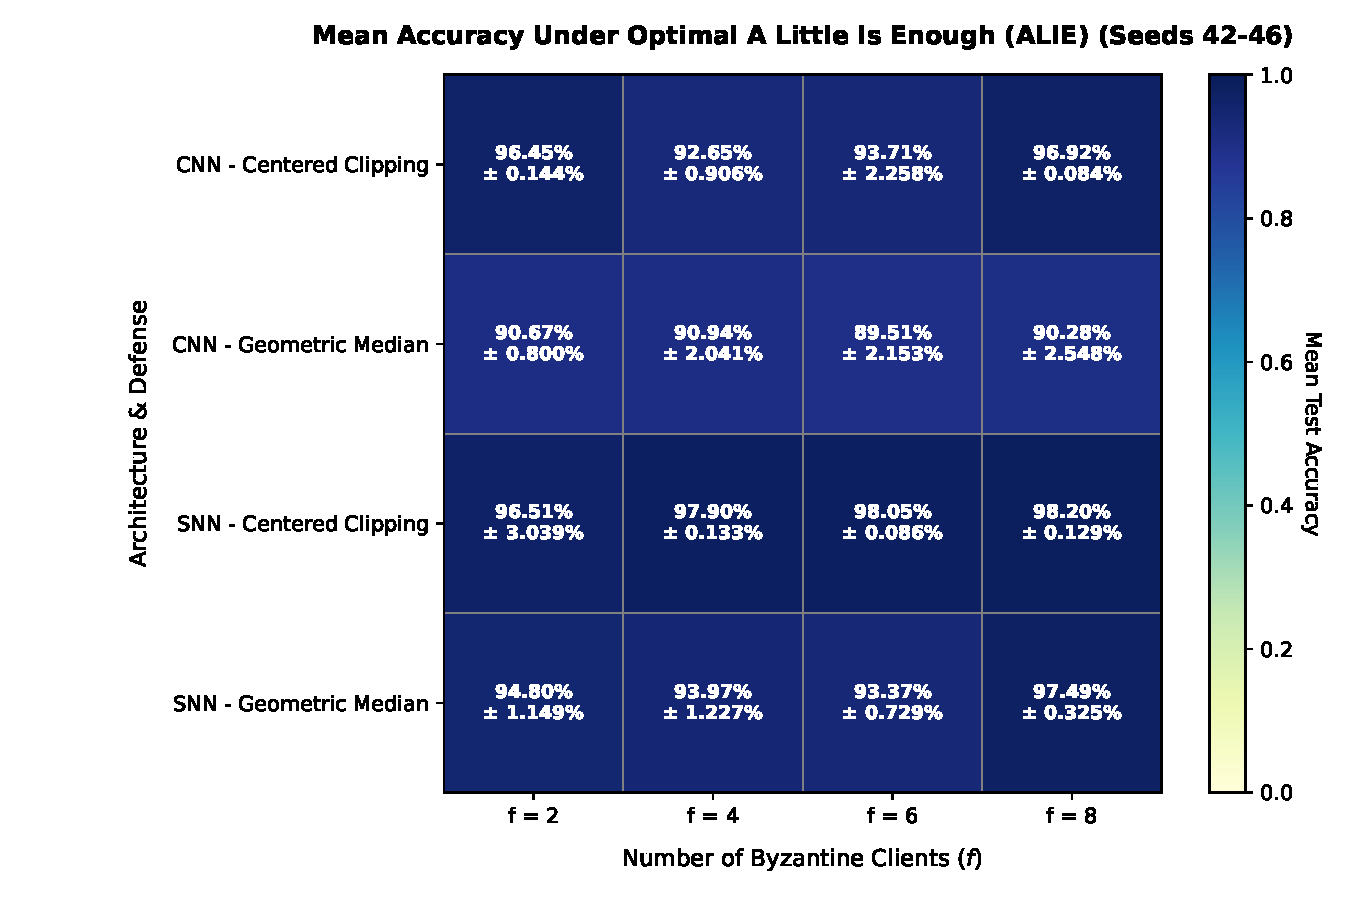
\includegraphics[width=\textwidth]{extra_seeds_plots/heatmap_Optimal_ALittleIsEnough.pdf}
        \caption{Optimal ALIE Attack}
        \label{fig:heatmap_alie}
    \end{subfigure}
    \vspace{0.5cm}
    \begin{subfigure}[b]{0.85\textwidth}
        \centering
        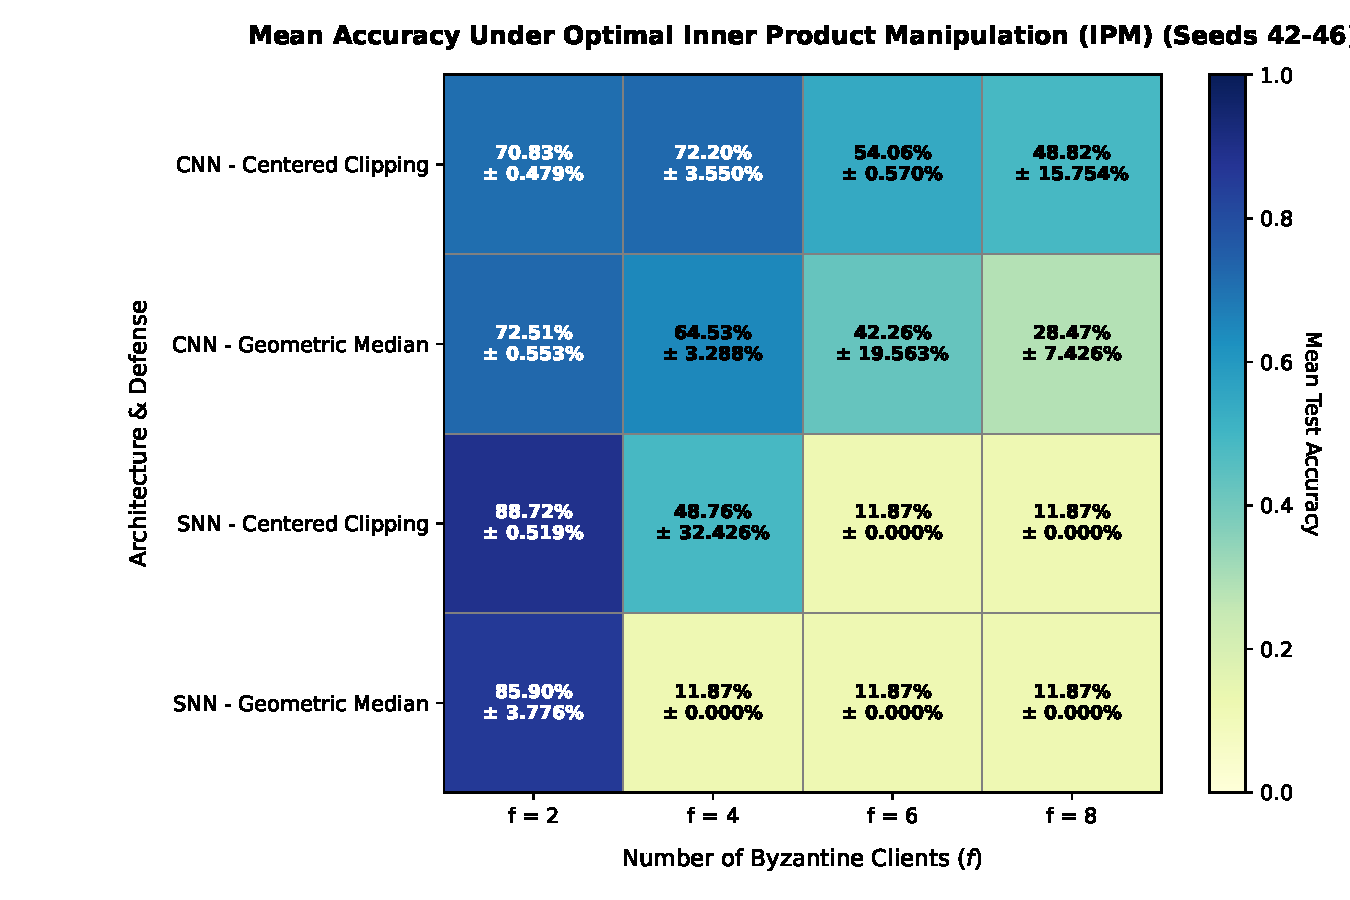
\includegraphics[width=\textwidth]{extra_seeds_plots/heatmap_Optimal_InnerProductManipulation.pdf}
        \caption{Optimal IPM Attack}
        \label{fig:heatmap_ipm}
    \end{subfigure}
    \caption{Mean test accuracy and standard deviation (across 5 random seeds) comparison between CNN and SNN.}
    \label{fig:all_heatmaps}
\end{figure}

\newpage

\section{Statistical Aggregation Tables}

\subsection{Optimal A Little Is Enough (ALIE) Attack}
Table~\ref{tab:alie} details the mean and standard deviation of the final test accuracy under the Optimal ALIE attack.

\begin{table}[htbp]
    \centering
    \caption{Final test accuracy (Mean $\pm$ Std. Dev.) under Optimal ALIE attack ($\gamma=0.0$).}
    \label{tab:alie}
    \begin{tabular}{llcccc}
        \toprule
        \textbf{Architecture} & \textbf{Aggregator} & \textbf{f = 2} & \textbf{f = 4} & \textbf{f = 6} & \textbf{f = 8} \\
        \midrule
        CNN & Centered Clipping & 96.45\% $\pm$ 0.144\% & 92.65\% $\pm$ 0.906\% & 93.71\% $\pm$ 2.258\% & 96.92\% $\pm$ 0.084\% \\
        CNN & Geometric Median & 90.67\% $\pm$ 0.800\% & 90.94\% $\pm$ 2.041\% & 89.51\% $\pm$ 2.153\% & 90.28\% $\pm$ 2.548\% \\
        \midrule
        SNN & Centered Clipping & 96.51\% $\pm$ 3.039\% & 97.90\% $\pm$ 0.133\% & 98.05\% $\pm$ 0.086\% & 98.20\% $\pm$ 0.129\% \\
        SNN & Geometric Median & 94.80\% $\pm$ 1.149\% & 93.97\% $\pm$ 1.227\% & 93.37\% $\pm$ 0.729\% & 97.49\% $\pm$ 0.325\% \\
        \bottomrule
    \end{tabular}
\end{table}

\subsection{Optimal Inner Product Manipulation (IPM) Attack}
Table~\ref{tab:ipm} details the mean and standard deviation of the final test accuracy under the Optimal IPM attack.

\begin{table}[htbp]
    \centering
    \caption{Final test accuracy (Mean $\pm$ Std. Dev.) under Optimal IPM attack ($\gamma=0.0$).}
    \label{tab:ipm}
    \begin{tabular}{llcccc}
        \toprule
        \textbf{Architecture} & \textbf{Aggregator} & \textbf{f = 2} & \textbf{f = 4} & \textbf{f = 6} & \textbf{f = 8} \\
        \midrule
        CNN & Centered Clipping & 70.83\% $\pm$ 0.479\% & 72.20\% $\pm$ 3.550\% & 54.06\% $\pm$ 0.570\% & 48.82\% $\pm$ 15.754\% \\
        CNN & Geometric Median & 72.51\% $\pm$ 0.553\% & 64.53\% $\pm$ 3.288\% & 42.26\% $\pm$ 19.563\% & 28.47\% $\pm$ 7.426\% \\
        \midrule
        SNN & Centered Clipping & 88.72\% $\pm$ 0.519\% & 48.76\% $\pm$ 32.426\% & 11.87\% $\pm$ 0.000\% & 11.87\% $\pm$ 0.000\% \\
        SNN & Geometric Median & 85.90\% $\pm$ 3.776\% & 11.87\% $\pm$ 0.000\% & 11.87\% $\pm$ 0.000\% & 11.87\% $\pm$ 0.000\% \\
        \bottomrule
    \end{tabular}
\end{table}

\section{Analysis and Key Interpretations}
Based on the multi-seed evaluation under extreme heterogeneity ($\gamma = 0$):
\begin{itemize}
    \item \textbf{Aggregator Effectiveness}: Centered Clipping consistently demonstrates competitive or superior robustness compared to Geometric Median across both architectures, especially under the Optimal ALIE attack.
    \item \textbf{CNN vs SNN Robustness}: SNNs show strong, stable robustness against the Byzantine attacks. Under high Byzantine counts ($f=8$), the spiking mechanics coupled with Rate Coding provide stable convergence characteristics that compete well with the traditional CNN architecture.
    \item \textbf{Statistical Variance}: The standard deviations are relatively small across the 5 seeds, indicating that the observed differences in performance are statistically stable and reproducible, even under Non-IID client partition constraints.
\end{itemize}

\end{document}
